\section{Dynamic Programming in Computational Biology}

Dynamic programming is one of the most commonly used algorithm design techniques in bioinformatics and computational biology. In this chapter, we discuss several problems of practical interest in computational biology that can be solve using dynamic programming. Dynamic programming is also the foundation of many more powerful algorithms such as BLAST (basic local alignment search tool). BLAST is probably one of the most used tool among biologists. It allows one to use a query string to search against a database of biological sequences, and return sequences that contains the query or are closely related to the query sequence. The core of any such algorithm is sequence alignment, which is solved using dynamic programming.

Bioinformatics is a subject as much about biology as it is about strings. Strings arise naturally as biological sequences. One of the most common thing to do with strings is comparing them. By comparing two strings and locating the common subsequence, we can find conserved protein motifs, infer evolutionary relationships, and even predicting function of newly discovered genes/proteins. We will look at DP algorithms that solve the so-called pairwise sequence alignment problem.

\section{Longest Common Subsequence}

Formally, given a sequence $X = x_1,x_2,\ldots, x_m$, the sequence $Z = z_1,z_2,\ldots,z_k$ is a subsequence of $X$ if there exists a strictly increasing sequence $i_1,i_2,\ldots,i_k$ of indicies such that for all $j = 1,2,\ldots,k$, we have $x_{i_j} = z_{j}$.

\section{Edit Distance}

\begin{figure}[htbp]
    \centering
    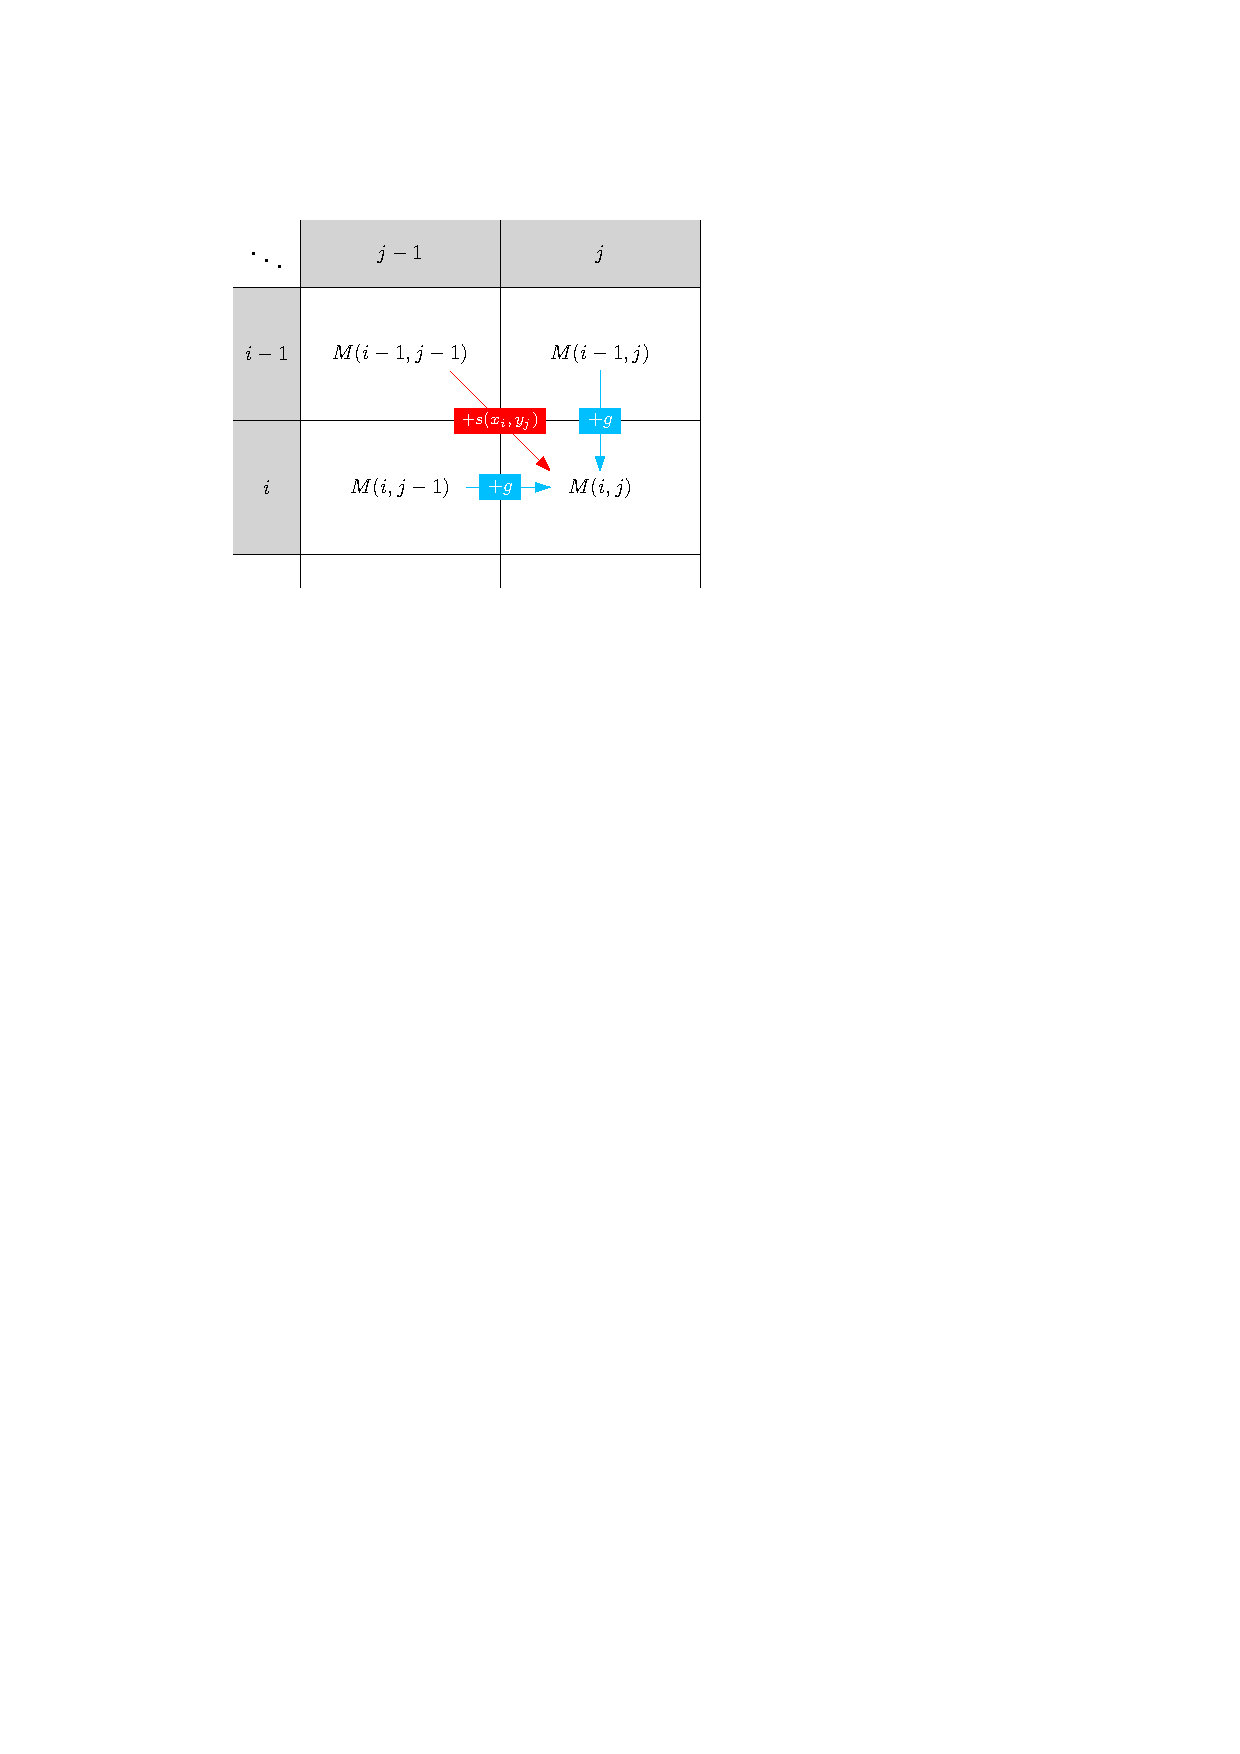
\includegraphics[width=0.4\linewidth]{dp/edit-distance.pdf}
    \caption{The dynamic programming matrix when computing the edit distance. Going diagonally corresponds to a match or substitution; going horizontally and vertically corresponds to insertion and/or deletion.}
    \label{fig:dp-editdistance-mat}
\end{figure}